\section{CU3 - Préparation des machines de TPs}

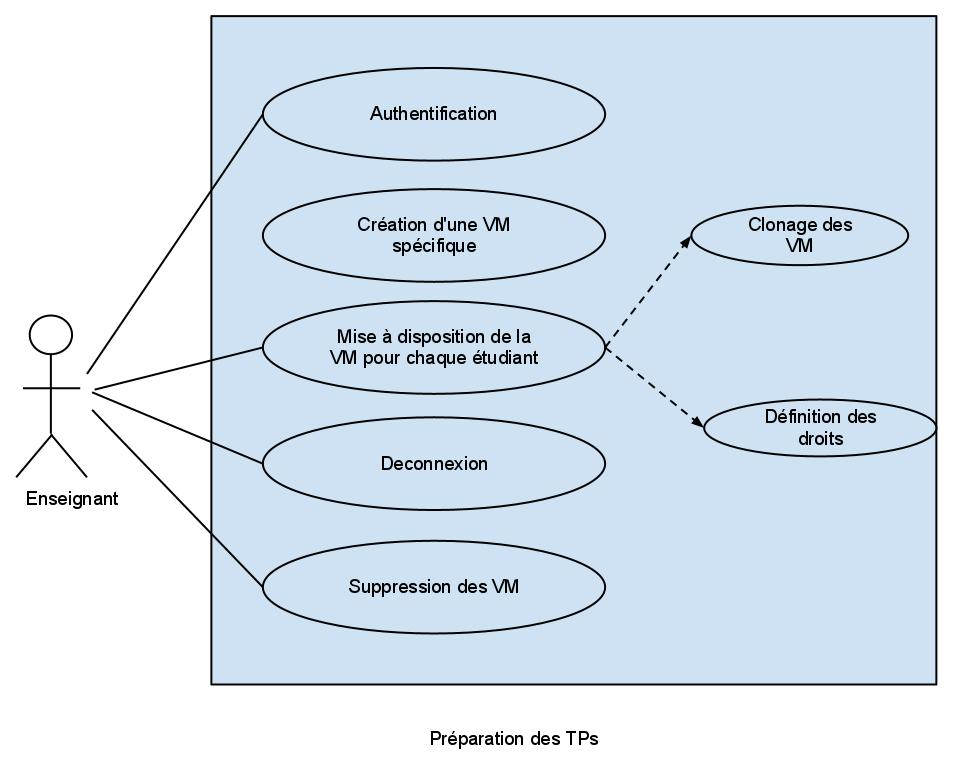
\includegraphics[scale=0.4]{CU3.jpg}

L’un des principaux avantages de cet outil technopédagogique est la souplesse qu’il procure dans la création et la diffusion de machines personnalisées pour des tâches spécifiques. Ainsi, il est très facile à un enseignant de créer des machines virtuelles spécialement pour un projet et de les fournir aux étudiants afin qu’ils puissent réaliser le travail demandé.
Au coeur de ce cas d’utilisation se trouve l’enseignant qui, en s’authentifiant sur le serveur d’infrastructure aura accès à une parc de machines virtuelles configurables. Il pourra alors en cloner une et la personnaliser afin de préparer les outils nécessaires à la réalisation du projet qu’il envisage de proposer aux étudiants. Une fois la machine prète, il lui sera également très aisé de la cloner de multiples fois afin d’en avoir suffisamment de copies pour tous les groupes d’étudiants. Il peut alors modifier les droits afin de restreindre l’accès aux machines de travail et permettre aux étudiants de travailler dans des conditions optimales. Suite à réalisation du travail par les étudiants (dont le déroulement est décrit en CU4), l’enseignant pourra supprimer les machines virtuelles de travail après correction.